\documentclass[twoside]{book}
\newif\ifpdf
\ifx\pdfoutput\undefined
\pdffalse % we are not running PDFLaTeX
\else
\pdfoutput=1 % we are running PDFLaTeX
\pdftrue
\fi
%\usepackage{times}
%\usepackage{amsmath}
\usepackage{calc}
\usepackage[latin1]{inputenc}
\usepackage{FFF}
\usepackage{amsfonts}
\usepackage{amsmath}
\usepackage{hyperref}
\usepackage{FFF}
\usepackage{makeidx}
\usepackage{color}
\usepackage{multicol}
\usepackage{graphicx}
%\usepackage{dessin}
\topmargin -1.54cm
\oddsidemargin 0cm   %marge a 2 cm
\evensidemargin 0cm  %marge a 2 cm
\newcommand{\indente}{\hbox to \parindent {\hss}}
\parindent 0cm
\headsep 0.5cm
\topskip .5cm
\footskip 1cm
\headheight 1.0cm
\textwidth  16.5cm
%  \parindent 0cm
\textheight 24cm
\def\freefempp{\texttt{freefem++ }}
\def\textRed{\color{red}}
\def\textBlack{\color{black}}
\def\Blue#1{\textcolor{blue}{#1}}
\def\Black#1{\textcolor{black}{#1}}
\def\Red#1{\textcolor{red}{#1}}
\def\Magenta#1{\textcolor{magenta}{#1}}
\def\hin{\hbox{ in }}
\def\hon{\hbox{ on }}
\def\Cpp{\texttt{C++~}}
\def\R{\mathrm{I\!R}}
\def\example{\textbf{Example:}}
\def\eq#1{\Blue{\[#1\]}}
\def\R{\mathbb{R}}
\def\Z{\mathbb{Z}}
\def\itemtt[#1]{ \item[\texttt{#1}]}
\def\plot[#1]#2#3{\begin{figure}[hbt]
\begin{center}
    \includegraphics*[#1]{#2}
\end{center}
\caption{\label{#2} #3}
\end{figure}
}
\def\Ostream{\texttt{ostream}}
\def\Istream{\texttt{istream}}
\def\Bool{\texttt{bool}}
\def\Real{\texttt{real}}
\def\Int{\texttt{int}}
\def\vecttwo#1#2{\left|\begin{smallmatrix} #1 \\ #2 \end{smallmatrix}\right.}
\def\vdeux(#1,#2){\left|\begin{smallmatrix} #1 \\ #2 \end{smallmatrix}\right.}
\def\HLINE#1{\hbox to \hsize {#1}}
\def\twoplot[#1]#2#3#4#5{
\begin{figure}[hbt]
\begin{multicols}{2}
\begin{center}
    \includegraphics*[#1]{#2}
    \caption{\label{#2} #4}
\end{center}
\begin{center}
    \includegraphics*[#1]{#3}
    \caption{\label{#3} #5}
\end{center}
\end{multicols}
\end{figure}
}% end twoplot macro
\newtheorem{remark}{\textbf{Remark}}
\newtheorem{bug}{\textbf{Bug:}}
\newtheorem{proposition}{\textbf{Proposition}}
\newtheorem{algorithm}{\textbf{Algorithm}}
\newenvironment{ttlist}
   {\begin{list}{}{\renewcommand{\makelabel}[1]{\texttt{##1}\hfil}%
        \setlength{\labelwidth}{3cm}
        \setlength{\leftmargin}{\labelwidth+\labelsep}
    }}%
   {\end{list}}


\begin{document}
\graphicspath{{./}{plots/}}
\ifpdf
\DeclareGraphicsExtensions{.pdf, .jpg, .tif}
\else
\DeclareGraphicsExtensions{.eps,.ps, .jpg}
\fi

\let\subsubsection\subsection
\let\subsection\section
\let\section\chapter



The domain $\Omega$ is defined with:

\bFF

real L=10;        //longueur du domaine                                    
real h=2.1;      // hauteur du bord gauche
real h1=0.35;    // hauteur du bord droite

//  maillage d'un tapeze
border a(t=0,L){x=t;y=0;};       // bottom:  $\Gamma_a$ \hfill              
border b(t=0,h1){x=L;y=t;};      // right:  $\Gamma_b$ \hfill    
border f(t=L,0){x=t;y=t*(h1-h)/L+h;}; //  free surface:  $\Gamma_f$ \hfill    
border d(t=h,0){x=0;y=t;};      // left:  $\Gamma_d$ \hfill 

int n=4;
mesh Th=buildmesh (a(10*n)+b(6*n)+f(8*n)+d(3*n));
plot(Th,ps="dTh.eps");
\eFF


\begin{figure}[hbt]
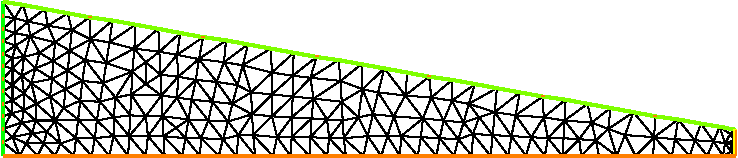
\includegraphics[width=15cm]{dTh}
\caption{The mesh of the domain $\Omega$}
\end{figure}

The free boundary problem is: 
 
Find $u$ and $\Omega$ such that:
$$ \left\{\begin{array}{cl}
 \displaystyle - \Delta u = 0  & \mbox{in } \Omega\\
\displaystyle      u = y         &\mbox{on } \Gamma_b \\
 \displaystyle      {\partial u  \over \partial n} = 0   &\mbox{on } \Gamma_d \cup \Gamma_a \\
 \displaystyle    {\partial u  \over \partial n} = { q\over K} n_x  
	        \mbox{\ and \ } {u = y}  &\mbox{on\ } \Gamma_ f
\end{array}\right. $$


We use a fixe point method;
$\Omega^0 = \Omega$

in two step, fist we solve the classical following problem:
$$ \left\{\begin{array}{rll} 
\displaystyle - \Delta u &= 0  & \mbox{in } \Omega^n\\
 \displaystyle      u &= y         &\mbox{on } \Gamma^n_b \\
\displaystyle      {\partial u  \over \partial n} &= 0   &\mbox{on } \Gamma^n_d \cup \Gamma^n_a\\
\displaystyle    u &= y        &\mbox{on\ } \Gamma^n_ f
\end{array}\right. $$

The varitional formulation is:

find $u$ on $V=H^1(\Omega^n)$, such than  $u=y$ on $\Gamma^n_b$ and $\Gamma^n_f$
$$
 \int_{\Omega^n}  \nabla u \nabla u' = 0,  \quad \forall u' \in V  \mbox{ with }  u' =0 \mbox{ on } 
\Gamma^n_b \cup \Gamma^n_f
$$
and secondly to construte a domain deformation $\mathcal{F}(x,y)=[x,y-v(x,y)]$ 

where $v$ is  solution of  the following problem: 

 $$ \left\{\begin{array}{rll}
\displaystyle - \Delta v &= 0  & \mbox{in } \Omega^n\\
 \displaystyle      v  &= 0         &\mbox{on } \Gamma^n_a \\
 \displaystyle      {\partial v \over \partial n} &= 0   &\mbox{on } \Gamma^n_b \cup \Gamma^n_d \\
\displaystyle    {\partial v  \over \partial n}  &=  \displaystyle {\partial u  \over \partial n} - { q\over K} n_x  
	          &\mbox{on\ } \Gamma^n_ f
\end{array}\right. $$

The varitional formulation is:

find $v$ on $V$, such than  $v=0$ on $\Gamma^n_a$ 
$$
 \int_{\Omega^n}  \nabla v \nabla v' = \int_{\Gamma_f^n}  ({\partial u  \over \partial n} - { q\over K} n_x )v',  \quad \forall v' \in V  \mbox{ with }  v' =0 \mbox{ on } 
\Gamma^n_a 
$$

finaly the new domain 
$\Omega^{n+1} = \mathcal{F}(\Omega^n)$



The  \texttt{FreeFem++} :implementation is:

\bFF

real q=0.02;      //flux entrant
real K=0.5;           //permeabilit�

fespace Vh(Th,P1);
int j=0;

Vh u,v,uu,vv;

problem Pu(u,uu,solver=CG) = int2d(Th)( dx(u)*dx(uu)+dy(u)*dy(uu)) 
  + on(b,f,u=y) ;

problem Pv(v,vv,solver=CG) = int2d(Th)( dx(v)*dx(vv)+dy(v)*dy(vv)) 
  +  on (a, v=0) + int1d(Th,f)(vv*((q/K)*N.y- (dx(u)*N.x+dy(u)*N.y))); 
  

real errv=1;
real erradap=0.001;
verbosity=1;
while(errv>1e-6)
{
  j++;       
  Pu;
  Pv;
  plot(Th,u,v ,wait=0);
  errv=int1d(Th,f)(v*v);
   real coef=1;

//  
  real mintcc = checkmovemesh(Th,[x,y])/5.; 
  real mint = checkmovemesh(Th,[x,y-v*coef]); 
  
  if (mint<mintcc ||  j%10==0) {  // mesh to bad => remeshing
    Th=adaptmesh(Th,u,err=erradap ) ;
    mintcc = checkmovemesh(Th,[x,y])/5.;     
  }
  
  while (1) 
  {  	    
    real mint = checkmovemesh(Th,[x,y-v*coef]); 
    
    if (mint>mintcc) break;
    
    cout << " min |T]  " << mint << endl;    
    coef /= 1.5;
  }
  
  Th=movemesh(Th,[x,y-coef*v]); // calcul de la deformation 
  cout << "\n\n"<<j <<"------------ errv = " << errv << "\n\n";

}
plot(Th,ps="d_Thf.eps");
plot(u,wait=1,ps="d_u.eps");
\eFF

\begin{figure}[hbt]
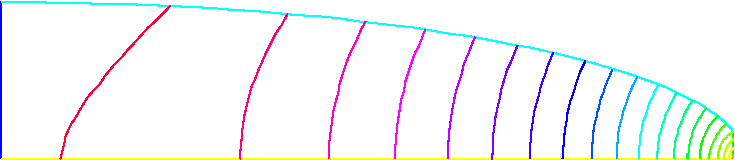
\includegraphics[width=15cm]{d_u}
\caption{The final solution on  the new  domain $\Omega^{72}$}
\end{figure}
\begin{figure}[hbt]
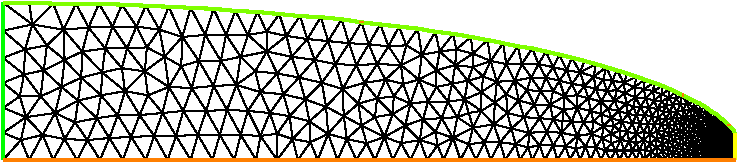
\includegraphics[width=15cm]{d_Thf}
\caption{The adapted mesh of the domain $\Omega^{72}$}
\end{figure}


\end{document}